\documentclass[10pt,twocolumn,letterpaper]{article}
\usepackage{cvpr}               % CVPR style
\usepackage{times}              % Font
\usepackage{graphicx}           % For including images
\usepackage{xcolor}             % For color customization in text
\usepackage{hyperref}           % For hyperlinks
\usepackage{amsmath}            % For mathematical formulas
\usepackage{caption}            % For customizing captions
\usepackage{multirow}           % For multi-row tables
\usepackage{array}

\hypersetup{
    colorlinks=true,
    linkcolor=blue,
    filecolor=magenta,      
    urlcolor=cyan,
}

\title{Machine Learning Coursework 2 Report: Autoencoders for Image Compression}
\author{Thomas Turner \\
University of Bath \\
}
\date{}

\begin{document}

\maketitle

\section{Introduction}

This paper explores and compares different autoencoder architectures for compressing and reconstructing images from a given dataset. The focus is primarily on optimizing visual reconstruction quality while minimizing the size of the compressed representations produced by each architecture.


%%%%%%%%%%%%%%%%%%%%%%%%%%%%%%%%%%%%%%%%%%%%%%%%%%%%%%%%%%%%%%%%%%%%%
\section{General Data Engineering}
The provided dataset is split in three subsets, containing a total of 1196 flattened images. Each flattened image is represented as a single row of 101,250 columns, where each entry holds a pixel component from the original image. The unflattened or reconstructed image dimensions are \texttt{150 x 225 x 3}, with three colour channels.
The first general data engineering technique employed was to load and concatenating the subsets to produce a complete dataset. Further, colour values for each channel were normalised, by casting them to a \texttt{float32} type, and scaling them to fit the range \texttt{[-1, 1]}. \texttt{Float32} is standard in modern deep learning due to its optimal balance between precision and memory efficiency, and scaling improves convergence rate and training stability as our gradients are less likely to grow arbitrarily large or small. The range \texttt{[-1, 1]} was selected based on our choice of activation function for both implemented models. See discussion in \textbf{Section 5.5} for further improvements upon and potential drawbacks of these considerations.

\section{Methodology}


\subsection{Architecture}
\begin{figure}[ht]
    \centering
    %%\includegraphics[width=0.5\textwidth]{example-image} % Replace with your image file
    \caption{Deep Convolutional Autoencoder Architecture}
    \label{fig:deep_convolutional_architecture}
\end{figure}

Figure \ref{fig:deep_convolutional_architecture} illustrates the architecture of a generic deep convolutional autoencoder. It includes an encoder block, which produces a compressed and deterministic latent vector, also known as the bottleneck. A decoder block reconstructs the image from this latent vector. The encoder employs a combination of convolutional and max pooling layers, the bottleneck is a single convolutional layer, and the decoder utilizes convolutional and spatial upsampling layers. Convolutional operations for all components of the model were chosen as they preserve spatial information, leading to improved reconstruction fidelity for images compared to fully connected architectures. Max pooling is utilised for downsampling as it is a widely adopted technique in state-of-the-art models such as AlexNet, however, in the last 10 years, the efficacy of max pooling layers has been questioned. For example, \cite{strivingforsimplicity} found that replacing max pooling layers with strided convolutions and nonlinearity retains accuracy on tasks such as image recognition, and improves the expressibility of the model. To address this issue, I implemented a second model using strided convolutions and compared their feature maps (Figure \ref{fig:strided-versus-pooling-feature-map-comparison}), and considered the impact of this result on final model selection (\textbf{Section 5.3}). An alternative approach for decoding makes use of convolutional transposes, but a heap of empirical evidence demonstrates they are likely to produce reconstruction defects such as checkerboard artifacts \cite{deconvolution}. Based on \cite{deconvolution}, a 'resize-convolution' scheme was implemented, building the decoder from pairs of convolutional and spatial upsampling layers, as described above.

\subsection{Training}

Nested cross-validation was used to train and select performant models, comprising an outer loop that partitions the dataset into $K_{outer}$ folds and an inner loop that subdivides each training set into $K_{inner}$ folds. Each of the inner folds were used for a hyperparameter optimisation process using the \texttt{Keras Tuner} framework, discussed more in the next section. Furthermore, relevant loss functions were used to evaluate reconstruction quality. Pixel-level reconstruction losses were first considered: mean squared error (MSE) and Huber loss. Huber loss extends MSE (and MAE) by including error bounds which account for outliers. The use of this loss for the final model was decided following an outlier detection experiment (Figure \ref{fig:reconstruction-loss-outlier-detection}). This analysis showed significant variability in the dataset, with a subset of images experiencing MSE reconstruction losses up to ten times worse than the mean average performance, highlighting the importance of addressing these outliers during the training process. Further, the Structural Similarity Index Measure (SSIM) was tested as a loss function. This is because it is likely to produce models with more visually appealing reconstructions, as a result of its prioritisation of higher-level features. This was tested in an experiment (Figure \ref{fig:cae-reconstruction-quality}), referred to and discussed in the next section. Adam was used as the optimisation algorithm. Considerations for tuning Adam are made in the next section. Batch normalization layers were used after every max pooling and upsampling process for the encoder and decoder respectively. This was in order to speed up convergence and improve stability of activation patterns in intermediate layers, ensuring that structural features were maintained and transferred to the bottleneck effectively.

\subsection{Hyperparameter Optimisation}

The initial hyperparameter under consideration was the pool size. The industry-standard choice of \texttt{(2,2)} was adopted, as it preserves spatial information across layers more effectively than more aggressive reduction strategies \cite{poolingmethods}. However, since the input image dimensions \texttt{150x225} are not divisible by 2, the following adjustments were implemented. A padding layer was prepended to the encoder, modifying the input dimensions to \texttt{(152, 232)}, the nearest factors of two. A cropping layer was appended to the decoder to restore the original input dimensions. Both replication padding and zero padding techniques were compared for both the initial and intermediate padding layers (Figure \ref{fig:reconstruction-quality-padding}). The next hyperparameter to consider was the choice of activation function in each layer. For all intermediate encoder and decoder layers, Leaky ReLU was used. This is in order to address the dying ReLU problem, where deeper activations become vanishingly small and are clipped to zero, preventing learning of meaningful compressed representations of the input image.  For the bottleneck, linear activation was used. This produces a continuous and unbounded latent space, allow us to preserve as much information as possible with limited bottleneck size. Finally, the reconstruction layer uses Hyperbolic Tangent to normalise pixel values in the range \texttt{[-1, 1]} to match the input image. To further resolve the dying ReLU problem, He initialisation was used. This prevents possible issues with poor early random weight initialisation, particularly where activations are too small or too large. For each convolutional layer, the minimal size odd-sized kernel \texttt{3x3} was used. This is because odd-sized kernels have a central element, and therefore symmetric receptive fields. This ensures no small shifts occur in pixel positions across convolutions which would otherwise lead to loss of spatial information.  Next, the number of convolutional layers, the number of filters per layer, and the bottleneck size were considered. Scaling the number of convolutional layers and filters increases the complexity and expressivity of the model, but may lead to overfitting. The bottleneck size, or the size of the compressed representation, can again lead to overfitting if too large but may also limit reconstruction quality if too small. To account for all of these tradeoffs, the \texttt{KerasTuner} framework for automatic hyperparameter optimisation was used. This framework was used within the nested cross-validation scheme. For each inner fold, a hyperparameter search is applied over a search space of possible models. The search space was defined by  the following constraints. Firstly, the encoder is limited to \texttt{1-3} pairs of convolutional and downsampling layers, and the decoder is organised symmetrically, with the same number of pairs of convolutions and upsampling layers. This constraint was justified based on the divisibility of 152 and 232, specifically, both are divisible up to eight times, therefore three downsamples with a pool size of \texttt{(2, 2)} before obtaining a fractional component. Further, the range  \texttt{[16, 32, 64]} was set for the number of filters in each convolutional layer, and the range \texttt{[8, 16, 32]} was set for the number of filters in the bottleneck layer. In practice, a tradeoff was made manually between reconstruction quality and compression ratio by re-training the best model configuration (Table \ref{tab:best-model-configuration}) with a reduced number of filters in the bottleneck layer, and comparing differences between these re-trained models and the original in the final visual reconstruction quality (Figure \ref{fig:reconstruction-loss-comparison}). See discussion in \textbf{Section 5.1} for how this approach could have been further improved. Hyperband was chosen for the corresponding hyperparameter search as it is highly resource-efficient, and intelligent in its focus on more promising model configurations. Further, [https://arxiv.org/abs/1603.06560] demonstrates its efficacy over traditional approaches such as random search, Bayesian optimisation and grid search. Three main parameters were considered for Hyperband, specifically, {factor}, {max\_epochs} and {hyperband\_iterations}. {max\_epochs}  is self-explanatory, it was set to 30 based on a combination of performance constraints and the results of an experiment shown and discussed in Figure \ref{fig:simple-convergence}. Factor reduces the number of models and the number of epochs are for each bracket in the Hyperband procedure. Standard choices range between 3 and 5. Five was selected to reduce training time, as 80\% of the model configurations in each training round will be discarded with this choice, and nested cross-validation is highly resource demanding, especially combined with the reasonably sized hyperparameter space for this model. The best model was selected using the mean average performance over all inner splits. Further, MSE, Huber loss and SSIM were used as validation losses in three separate experiments with the same training scheme, and the final visual reconstruction quality was compared in Figure \ref{fig:cae-reconstruction-quality}. The values of $K_{inner} = 3$ and $K_{outer} = 10$ were selected based on industry standards but also performance constraints.  Empirical evidence demonstrates that the default and widely used values $\alpha = 0.001, $ $\beta_{1} = 0.9, $ $\beta_{2} =  0.999$ for the Adam optimiser are sufficient and stable, and further the algorithm adapts during training. 



\section{Experiments, Results and Discussion}

Figure \ref{fig:reconstruction-loss-outlier-detection} displays the distribution of MSE reconstruction losses for the best model configuration (Table \ref{tab:best-model-configuration}) evaluated on a randomly selected sample of 200 images. This demonstrates a large variability in reconstruction losses and a peak in loss at approximately 0.03, ten times less accurate than the main bulk of reconstructions. This demonstrates the necessity to use Huber loss, a less outlier-sensitive loss function, during the training process. 

In Figure \ref{fig:simple-convergence}, a simple model configuration was trained using an 80-20 train-test split, and it was found that the Huber loss for this model, averaged over a batch size of 32, converged consistently at the 50th to the 55th epoch. However, minimal improvements are seen after the 35th epoch. These considerations indicate that the Hyperband max\_epochs parameter should be selected between 30 and 50.

Figure \ref{fig:strided-versus-pooling-feature-map-comparison} trains two best model configurations, one replaced with strided convolutions for downsampling. Activation heatmaps are then extracted and superimposed over image reconstructions to compare spatial feature representation and focus.

\begin{table}[ht]
\centering
\begin{tabular}{|l|m{5cm}|}
\hline
\textbf{Layer} & \textbf{Description} \\
\hline
Input Layer & The original input data to the encoder. \\
\hline
Encoder & Padding 1 pixel at the bottom and top, padding 3 pixels to the left and 4 to the right. Conv2D layer with 64 filters and kernel size \texttt{3x3},  MaxPooling2D layer with pool size \texttt{2x2}, BatchNormalization layer, Conv2D layer with 32 filters and same kernel size, MaxPooling2D layer with same pool size as before., BatchNormalization layer.\\
\hline
Bottleneck & Conv2D layer with 32 filters, kernel size \texttt{3x3}.\\
\hline
Decoder & Conv2D layer with 32 filters, kernel size \texttt{3x3}. UpSampling2D layer by size \texttt{2x2}. BatchNormalization layer. Conv2D layer with 64 filters and same kernel size as before. UpSampling2D layer by same size as before. BatchNormalization layer. Conv2D layer with 3 filters for 3 channels and same kernel size before. Final cropping layer by same quantities as initial padding. \\
\end{tabular}
\caption{Configuration of best model selected using nested cross validation and Hyperband tuning.}
\label{tab:best-model-configuration}
\end{table}



\begin{figure}[ht]
    \centering
    %%\includegraphics[width=0.5\textwidth]{example-image} % Replace with your image file
    \caption{Activation heatmap comparison between stride-based and pooling-based downsampling}
    \label{fig:strided-versus-pooling-feature-map-comparison}
\end{figure}


\begin{figure}[ht]
    \centering
    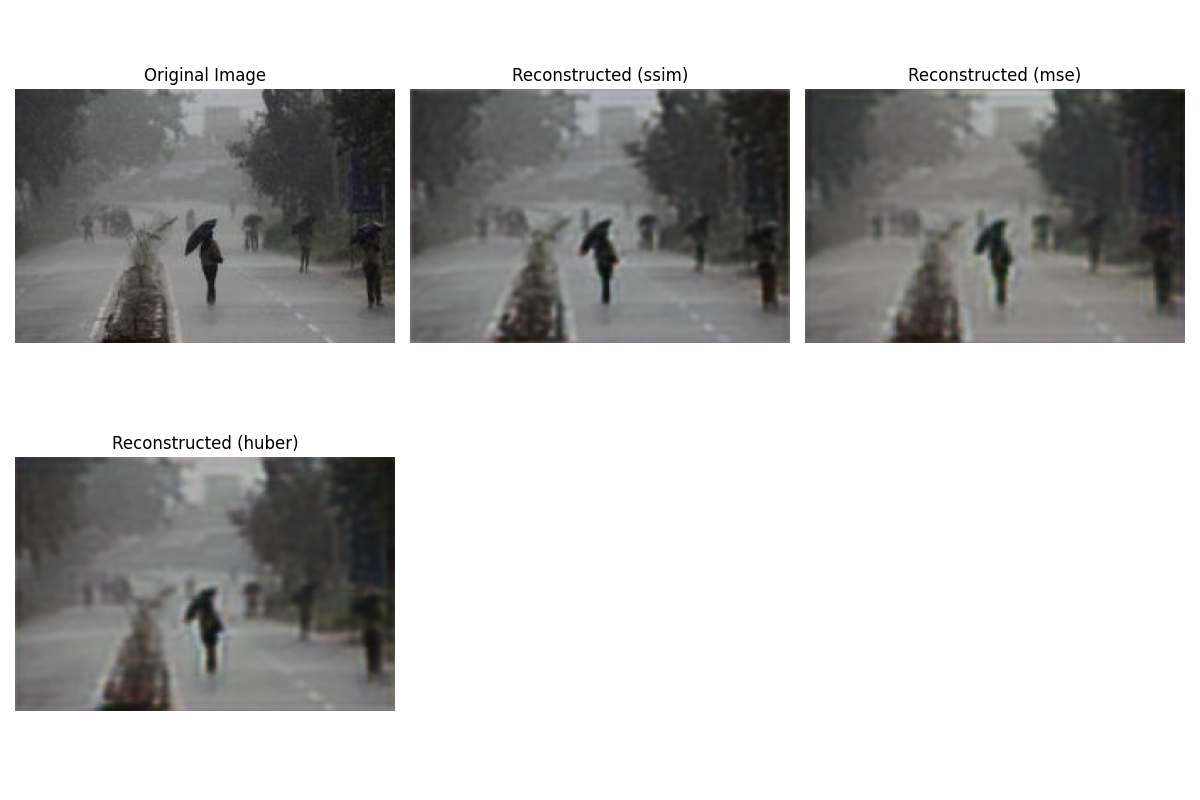
\includegraphics[width=0.5\textwidth]{ReconstructionQualityComparisons2.png} 
    \caption{Visual reconstruction quality of best CAE models from nested cross validation using MSE, Huber Loss and SSIM.}
    \label{fig:cae-reconstruction-quality}
\end{figure}

\begin{figure}[ht]
    \centering
    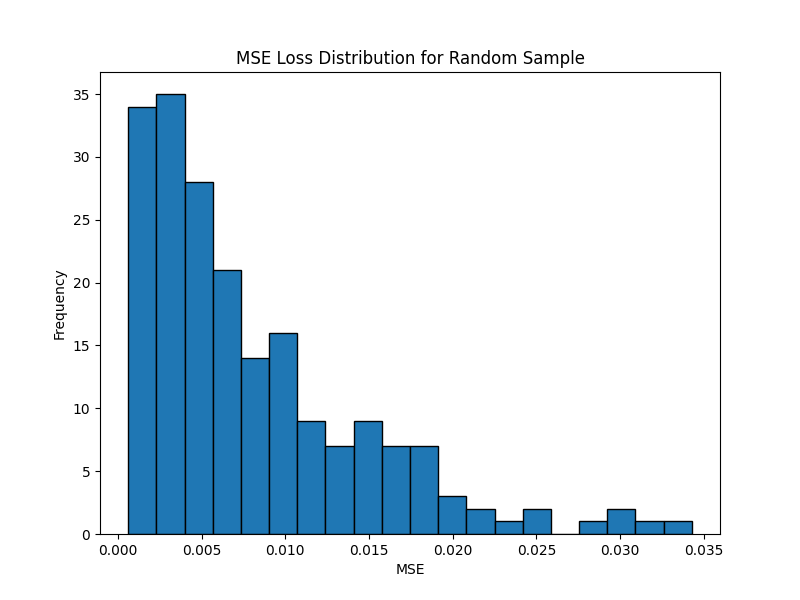
\includegraphics[width=0.3\textwidth]{MSEReconstructionLossDistribution.png} % Replace with your image file
    \caption{Histogram of MSE reconstruction losses for best model configuration.}
    \label{fig:reconstruction-loss-outlier-detection}
\end{figure}

\begin{figure}[ht]
    \centering
    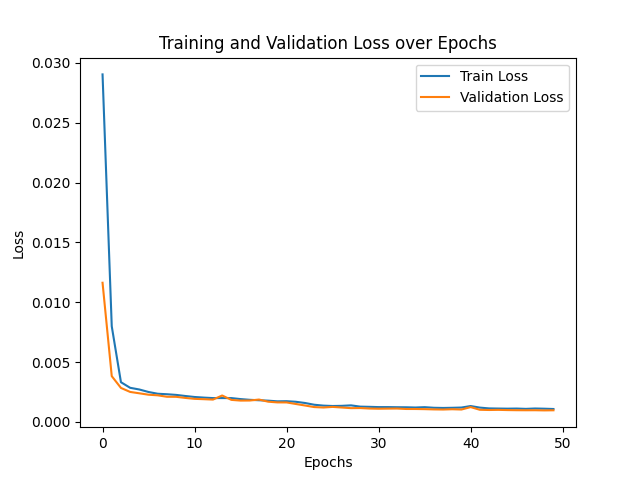
\includegraphics[width=0.3\textwidth]{Convergence.png} % Replace with your image file
    \caption{Convergence of simple model on single train-test split.}
    \label{fig:simple-convergence}
\end{figure}

\begin{figure}[ht]
    \centering
    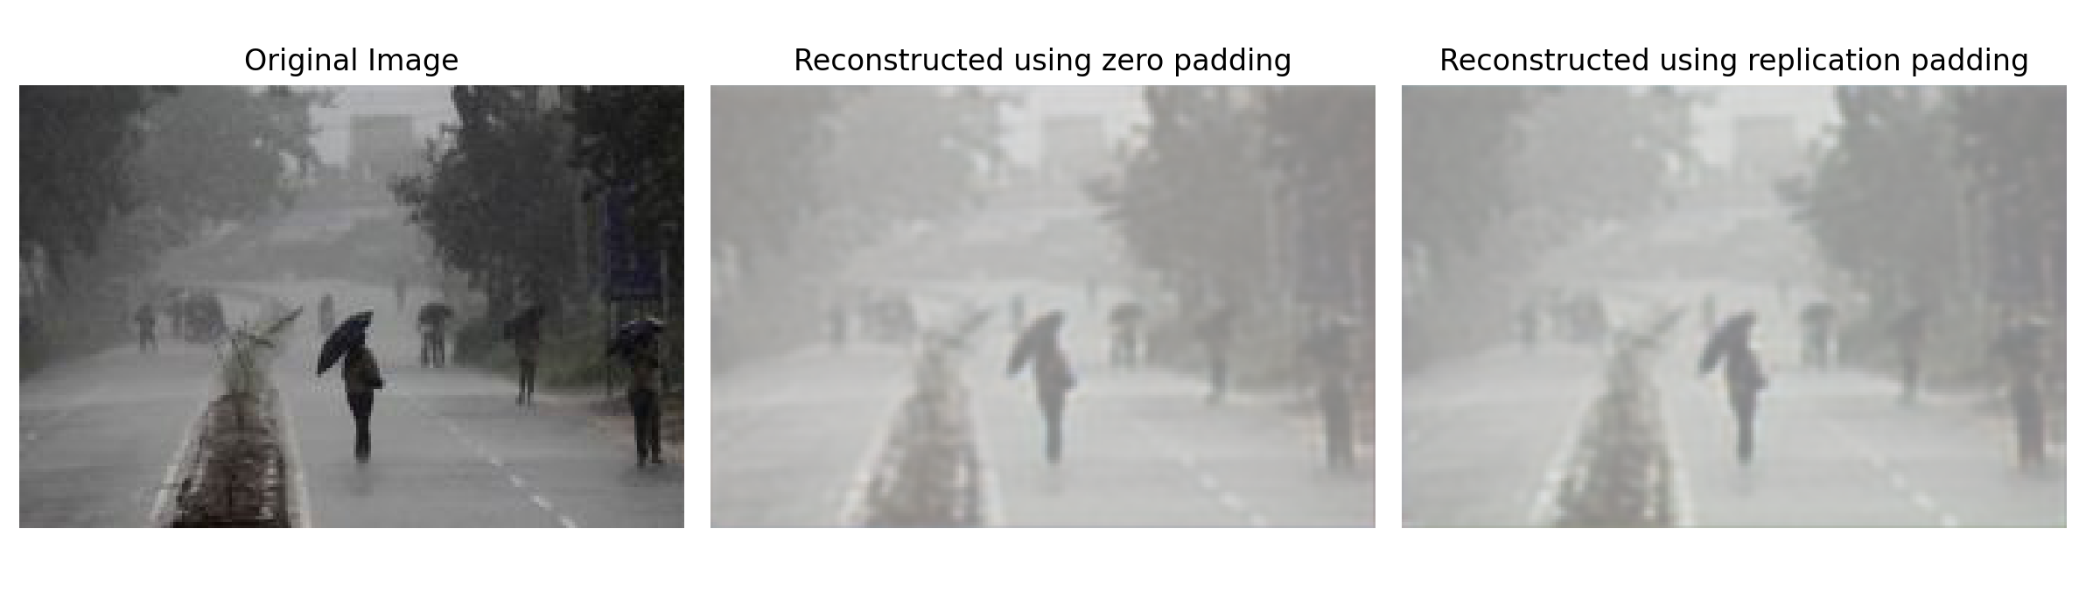
\includegraphics[width=0.5\textwidth]{PaddingReconstructions.png} 
    \caption{Visual reconstruction quality of zero-padding versus replication padding using simple model.}
    \label{fig:reconstruction-quality-padding}
\end{figure}

\begin{figure}[ht]
    \centering
    %%\includegraphics[width=0.5\textwidth]{example-image} % Replace with your image file
    \caption{Comparison of best model with varying bottleneck sizes. Compression ratios are labelled for each reconstructed image, calculated based on the size of the bottleneck depending on the number of filters selected.}
    \label{fig:reconstruction-loss-comparison}
\end{figure}


\begin{figure}[ht]
    \centering
    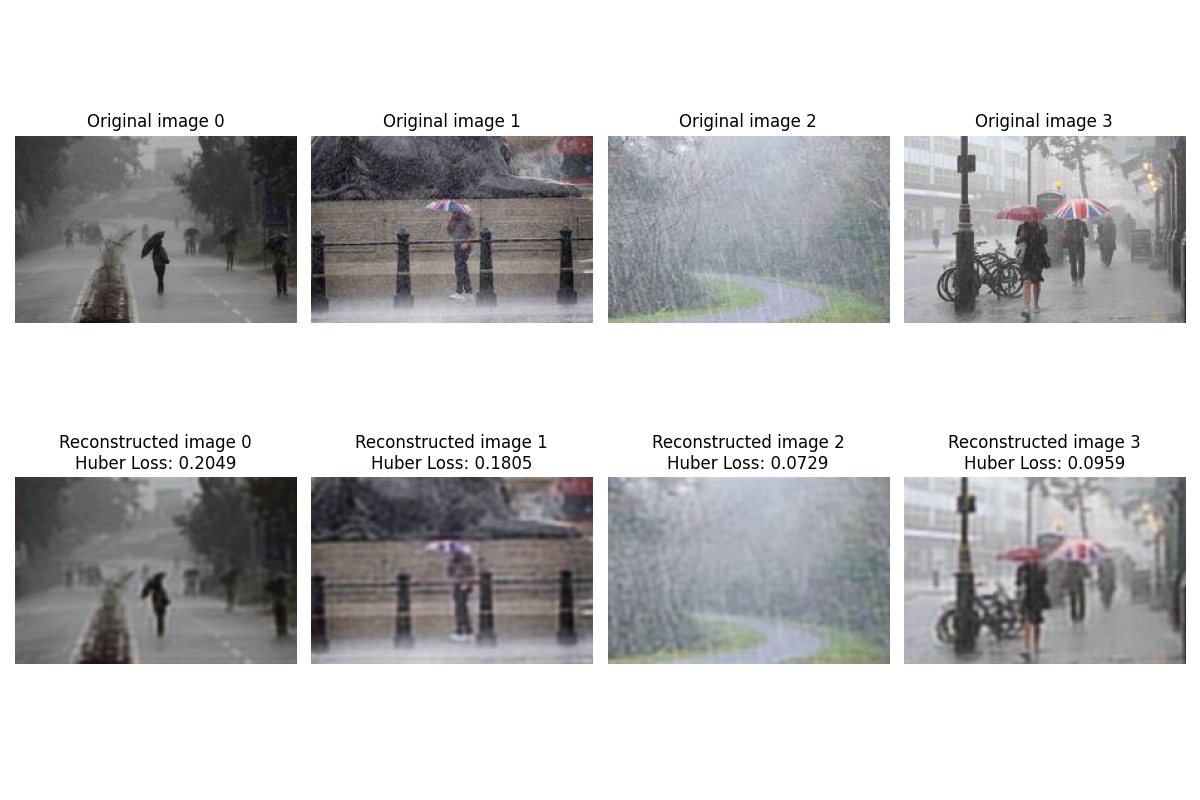
\includegraphics[width=0.5\textwidth]{ReconstructionQualityComparisons3.png} 
    \caption{Display of four reconstructions and associated Huber loss from best model configuration.}
    \label{fig:reconstructions}
\end{figure}


\section{Conclusions and Further Improvements}


\subsection{Bottleneck Regularisation}

In the training process I outlined, the bottleneck is a single convolutional layer, or equivalently, a compressed feature map. The size of this bottleneck depends on the output dimensions of previous downsampling operations and the number of filters in the convolution. Therefore, the range of filter values passed to Hyperband was small and limited (\texttt{[8, 16, 32]}), however, a specific choice of filter value was only preferred during optimisation if it contributed to a better loss score. Hyperband selected the best model configuration with 32 filters in the bottleneck, but this suffers from a higher compression ratio (Figure \ref{fig:reconstruction-loss-comparison}). In order to account for this, it would be reasonable to include the bottleneck size as a regularisation term added to the loss. This would strike a balance between reconstruction quality and bottleneck size, as models with higher bottleneck sizes would be penalised, depending on the weight of the regularisation term.

\subsection{Wavelet Preprocessing}

\ref{wavelet-decomposition} discusses an extension to the standard CAE architecture incorporating wavelet transforms for each colour channel, and a parallel training scheme for each channel. This produced high reconstruction quality and better compression measured by bitrate coding (per pixel), and also dramatically improved training time. Wavelet decomposition in particular could have been included as a pre-processing step, particularly for improving compression as these transforms are capable of representing visual features at multiple scales with a small number of coefficients.

\subsection{Strided Versus Pooling-Based Downsampling}

 
\subsection{VQ-CVAE}

CVAE (Convolutional Variational Autoencoder) and VQ-CVAE (Vector-Quantised Convolutional Variational Autoencoder) are alternative architectures that were considered during the model selection and development process. Specifically, it is difficult to increase the compression ratio significantly in a standard convolutional autoencoder without using a fully connected layer for the bottleneck. This is problematic as important spatial information will be lost in flattening the image representation. CVAE can overcome this issue by encoding the latent space as a multivariate Gaussian distribution, using fully connected layers for the mean and variance of this distribution, effectively compacting each latent vector and then regenerating spatial features in the sampling process. VQ-(C)VAE approaches were introduced and demonstrated in the work by [Van den Oord et al. (2017) Neural Discrete Representation Learning]. VQ-VAE improves compression by discretizing the continuous latent space into a finite set of codebook entries, reducing the redundancy of the latent representations . In theory and future development, the usage of both of these architectures may have resulted in a higher compression ratio while maintaining a high level of image reconstruction quality.


\subsection{Other Data Engineering}


%%%%%%%%%%%%%%%%%%%%%%%%%%%%%%%%%%%%%%%%%%%%%%%%%%%%%%%%%%%%%%%%%%%%%
% References
%%%%%%%%%%%%%%%%%%%%%%%%%%%%%%%%%%%%%%%%%%%%%%%%%%%%%%%%%%%%%%%%%%%%%
\begin{thebibliography}{9}

\bibitem{deconvolution}
Odena, A., Dumoulin, V., \& Olah, C. (2016). Deconvolution and Checkerboard Artifacts. \textit{Distill}. \href{https://doi.org/10.23915/distill.00003}{https://doi.org/10.23915/distill.00003}.

\bibitem{strivingforsimplicity}
Springenberg, J. T., Dosovitskiy, A., Brox, T., Riedmiller, M. (2014). Striving for Simplicity: The All Convolutional Net. 

\bibitem{poolingmethods}
Gholamalinezhad, H., Khosravi, H. (2020). Pooling Methods in Deep Neural Networks, a Review. 

\bibitem{wavelet-decomposition}
Akyazi, P. and Ebrahimi, T. (2019). Learning-based image compression using convolutional autoencoder and wavelet decomposition. *Proceedings of the CVPRW 2019*. Available at: \url{https://openaccess.thecvf.com/content\_CVPRW\_2019/html/CLIC\_2019/Akyazi\_Learning-Based\_Image\_Compression\_using\_Convolutional\_Autoencoder\_and\_Wavelet\_Decomposition\_CVPRW\_2019\_paper.html} (Accessed: 19 March 2025).

\end{thebibliography}

%%%%%%%%%%%%%%%%%%%%%%%%%%%%%%%%%%%%%%%%%%%%%%%%%%%%%%%%%%%%%%%%%%%%%
% Appendix
%%%%%%%%%%%%%%%%%%%%%%%%%%%%%%%%%%%%%%%%%%%%%%%%%%%%%%%%%%%%%%%%%%%%%
\appendix

\section{Appendix}
Include extra screenshots of code snippets or experimental results or further experimental results that couldn’t fit into the main report due to space constraints.

\end{document}
